% -*- coding: utf-8 -*-
% !TEX program = xelatex

\documentclass[9pt]{beamer}

\usetheme[style=beta]{epyt} % alpha, beta, delta, gamma, zeta
% \usetheme{Warsaw}
\usepackage[UTF8,noindent]{ctex}
\def\blue{\textcolor{blue}}
\def\red{\textcolor{red}}
\def\purple{\textcolor{purple}}
\def\ds{\displaystyle}
\def\cd{\cdots}
\def\dd{\ddots}
\def\vd{\vdots}
\def\id{\iddots}
\def\ft{\frametitle}
\def\diag{\mathrm{diag}}

\def\A{\boldsymbol{A}}
\def\B{\boldsymbol{B}}
\def\C{\boldsymbol{C}}
\def\D{\boldsymbol{D}}
\def\E{\boldsymbol{E}}
\def\F{\boldsymbol{F}}
\def\T{\boldsymbol{T}}
\def\U{\boldsymbol{U}}
\def\X{\boldsymbol{X}}
\def\Y{\boldsymbol{Y}}
\def\Z{\boldsymbol{Z}}
\def\QQ{\boldsymbol{Q}}

\def\R{\mathbb R}
\def\rank{\mathrm{R}}
\def\det{\mathrm{det}}
\def\nn{{\boldsymbol{n}}}
\def\xx{{\boldsymbol{x}}}
\def\yy{{\boldsymbol{y}}}
\def\aa{{\boldsymbol{a}}}
\def\bb{{\boldsymbol{b}}}
\def\ee{{\boldsymbol{e}}}
\def\ii{{\boldsymbol{i}}}
\def\jj{{\boldsymbol{j}}}
\def\kk{{\boldsymbol{k}}}
\def\uu{{\boldsymbol{u}}}
\def\vv{{\boldsymbol{v}}}

\def\tf{\ttfamily}
\def\zero{\boldsymbol{0}}
\def\II{\boldsymbol{I}}
\def\PP{\boldsymbol{P}}
\def\XX{\boldsymbol{X}}
\def\Lambdabd{\boldsymbol{\Lambda}}
\def\alphabd{\boldsymbol{\alpha}}
\def\betabd{\boldsymbol{\beta}}
\def\gammabd{\boldsymbol{\gamma}}
\def\xibd{\boldsymbol{\xi}}
\def\etabd{\boldsymbol{\eta}}
\def\epsilonbd{\boldsymbol{\epsilon}}
\usepackage{multicol}
%\usepackage{fontspec}
\usepackage[most]{tcolorbox}
\newcounter{testexample}
\usepackage{xparse}
\usepackage{lipsum}
\usepackage[UTF8,noindent]{ctex}
\usepackage{extarrows}
%\usepackage{courier}
\usepackage{animate}
\usepackage{dcolumn}
\usepackage{pgf}
\usepackage{tikz}
\usetikzlibrary{calc}
\usetikzlibrary{arrows,snakes,backgrounds,shapes,patterns}
\usetikzlibrary{matrix,fit,positioning,decorations.pathmorphing}
\usepackage{listings}
\lstset{
        language=python,
        keywordstyle=\color{blue!70},
        frame=single,
        basicstyle=\ttfamily,
        commentstyle=\color{red},
        breakindent=0pt,
        rulesepcolor=\color{red!20!green!20!blue!20},
        rulecolor=\color{black},
        tabsize=4,
        numbersep=5pt,
        breaklines=true,
        %% backgroundcolor=\color{red!10},
        showstringspaces=false,
        showspaces=false,
        showtabs=false,
        extendedchars=false,
        escapeinside=``,
        frame=single,
}
\def\exampletext{例} % If English
\NewDocumentEnvironment{testexample}{ O{} }
{
\colorlet{colexam}{red!55!black} % Global example color
\newtcolorbox[use counter=testexample]{testexamplebox}{%
    % Example Frame Start
    empty,% Empty previously set parameters
    title={\exampletext: #1},% use \thetcbcounter to access the testexample counter text
    % Attaching a box requires an overlay
    attach boxed title to top left,
       % Ensures proper line breaking in longer titles
       minipage boxed title,
    % (boxed title style requires an overlay)
    boxed title style={empty,size=minimal,toprule=0pt,top=4pt,left=3mm,overlay={}},
    coltitle=colexam,fonttitle=\bfseries,
    before=\par\medskip\noindent,parbox=false,boxsep=0pt,left=3mm,right=0mm,top=2pt,breakable,pad at break=0mm,
       before upper=\csname @totalleftmargin\endcsname0pt, % Use instead of parbox=true. This ensures parskip is inherited by box.
    % Handles box when it exists on one page only
    overlay unbroken={\draw[colexam,line width=.5pt] ([xshift=-0pt]title.north west) -- ([xshift=-0pt]frame.south west); },
    % Handles multipage box: first page
    overlay first={\draw[colexam,line width=.5pt] ([xshift=-0pt]title.north west) -- ([xshift=-0pt]frame.south west); },
    % Handles multipage box: middle page
    overlay middle={\draw[colexam,line width=.5pt] ([xshift=-0pt]frame.north west) -- ([xshift=-0pt]frame.south west); },
    % Handles multipage box: last page
    overlay last={\draw[colexam,line width=.5pt] ([xshift=-0pt]frame.north west) -- ([xshift=-0pt]frame.south west); },%
    }
\begin{testexamplebox}}
{\end{testexamplebox}\endlist}


\renewcommand{\proofname}{\textbf{证明}}
\newtheorem{li}{例}
\newtheorem*{li*}{例}
\newtheorem{lianxi}{练习}
\newtheorem{jielun}{结论}
\newtheorem{dingli}{定理}
\newtheorem*{dingli*}{定理}
\newtheorem{mingti}{{命题}} 
\newtheorem{yinli}{{引理}} 
\newtheorem{tuilun}{{推论}}
\newtheorem{dingyi}{{定义}}
\newtheorem*{dingyi*}{{定义}} 
\newtheorem*{jie}{{解}}
\newtheorem*{zhengming}{{证明}}
\newtheorem{zhu}{{注}}
\newtheorem*{zhu*}{{注}}
\newtheorem{xingzhi}{{性质}}
\newtheorem{wenti}{{问题}}
\newtheorem{rem}{{Remark}}
\newtheorem{lem}{{Lemma}}



\begin{document}

\title{数据结构与算法}
\subtitle{算法分析}
\author{张晓平}
\institute{武汉大学数学与统计学院}


\begin{frame}[plain]\transboxout
  \titlepage
\end{frame}

\section*{目录}
\frame{  
  \frametitle{\secname}
  \begin{multicols}{2}  %两行目录
    \tableofcontents
  \end{multicols}
}
\AtBeginSection[] {  %在每个subsection前面显示一次目录
  \frame{
    \begin{multicols}{2}  %两行目录
      \tableofcontents[current,currentsection]
    \end{multicols}
  }
}

\AtBeginSubsection[] {  %在每个subsection前面显示一次目录
  \frame{
    \begin{multicols}{2}  %两行目录
      \tableofcontents[current,currentsubsection]
    \end{multicols}
  }
}


\section{目标}
\begin{frame}\ft{\secname}
\begin{itemize}
\item 理解算法分析的重要性
\item 能够使用大 O 符号描述算法执行时间
\item 理解 Python 列表和字典的常见操作的大 O 执行时间
\item 理解 Python 数据的实现是如何影响算法分析的。
\item 了解如何对简单的 Python 程序做基准测试(benchmark)。
\end{itemize}
\end{frame}

\section{快速开始}



自计算机通过电缆和交换机来传递人的指令起,人们对编程的看法就发生了许多变化。与社会的许多方面一样,计算技术的变化为计算机科学家提供了越来越多的工具和平台来实践他们的工艺。计算机的快速发展,诸如快速处理器、高速网络和大容量存储器已经让计算机科学家陷入高度复杂螺旋中。在所有这些快速演变中,一些基本原则保持不变。计算机科学关注用计算机来解决问题。


或许你花了很多时间学习了解决问题的基础知识,希望自己能把问题弄清楚并提出解决方案。接着你可能还会发现编程有些难。问题以及解决方案的复杂性可能会掩盖求解过程中的一些基本思想。



本章的其余部分将着重介绍两个重要的领域。首先回顾一下计算机科学与研究算法和数据结构所必须适应的框架,特别是我们需要研究这些主题的原因,以及如何理解这些主题有助于我们更好的解决问题。其次我们将回顾 Python 编程语言。这里不提供详尽的参考,但我们将在其余章节中给出基本数据结构的示例和解释。 

\section{什么是计算机科学}

Computer science is often difficult to define. This is probably due to the unfortunate use of the word “computer” in the name. As you are perhaps aware, computer science is not simply the study of computers. Although computers play an important supporting role as a tool in the discipline, they are just that–tools.

计算机科学不好定义,由于在名字中有“计算机”一词。然而,计算机科学并非简单地研究计算机,尽管计算机作为一种工具在学科中发挥重要的支持作用,但它们只是工具。

Computer science is the study of problems, problem-solving, and the solutions that come out of the problem-solving process. Given a problem, a computer scientist’s goal is to develop an algorithm, a step-by-step list of instructions for solving any instance of the problem that might arise. Algorithms are finite processes that if followed will solve the problem. Algorithms are solutions.

计算机科学研究问题、解决问题并生成解决问题的方案。给定一个问题,计算机科学家的目标是开发一个算法,一系列的指令列表,用于解决可能出现的问题。算法遵循它有限的过程就可以解决问题。

Computer science can be thought of as the study of algorithms. However, we must be careful to include the fact that some problems may not have a solution. Although proving this statement is beyond the scope of this text, the fact that some problems cannot be solved is important for those who study computer science. We can fully define computer science, then, by including both types of problems and stating that computer science is the study of solutions to problems as well as the study of problems with no solutions.

计算机科学可以被认为是对算法的研究。但是,我们必须清楚地认识到,一些问题可能没有解决方案。虽然证明这种说法正确性超出了本文的范围,但一些问题不能解决的事实对于那些研究计算机科学的人是很重要的。可以这么说,计算机科学研究有解决方案和没有解决方案的问题。

It is also very common to include the word computable when describing problems and solutions. We say that a problem is computable if an algorithm exists for solving it. An alternative definition for computer science, then, is to say that computer science is the study of problems that are and that are not computable, the study of the existence and the nonexistence of algorithms. In any case, you will note that the word “computer” did not come up at all. Solutions are considered independent from the machine.

当描述问题及其解决方案时,会提到计算一词。若存在一个算法解决某个问题,就称该问题是可计算的。计算机科学的另一个定义是:计算机科学是研究那些可计算和不可计算的问题,研究是不是存在一种算法来解决它。请注意这里没有涉及到“计算机”一词,解决方案与机器无关。

Computer science, as it pertains to the problem-solving process itself, is also the study of abstraction. Abstraction allows us to view the problem and solution in such a way as to separate the so-called logical and physical perspectives. The basic idea is familiar to us in a common example.

计算机科学,因涉及问题解决过程本身,是关于抽象的研究。抽象使我们能从逻辑视角和物理视角来分别看待问题及解决方案。基本思想跟我们常见的例子一样。

Consider the automobile that you may have driven to school or work today. As a driver, a user of the car, you have certain interactions that take place in order to utilize the car for its intended purpose. You get in, insert the key, start the car, shift, brake, accelerate, and steer in order to drive. From an abstraction point of view, we can say that you are seeing the logical perspective of the automobile. You are using the functions provided by the car designers for the purpose of transporting you from one location to another. These functions are sometimes also referred to as the interface.

假设你开车上学或上班。作为司机,也就是汽车的用户,你为了让汽车载你到目的地,你会和汽车有些互动,如上汽车、插钥匙、点火、换挡、制动、加速和转向。从抽象的角度,你所看到的是汽车的逻辑视角。你使用的是汽车设计者提供的功能,将你从一个地方载到另一个地方。这些功能有时也被称为接口。

On the other hand, the mechanic who must repair your automobile takes a very different point of view. She not only knows how to drive but must know all of the details necessary to carry out all the functions that we take for granted. She needs to understand how the engine works, how the transmission shifts gears, how temperature is controlled, and so on. This is known as the physical perspective, the details that take place “under the hood.”

另一方面,汽车修理师傅则有一个截然不同的视角。他不仅知道如何开车,还必须知道所有必要的细节,使我们认为理所当然的功能运行起来。他需要了解发动机如何工作、变速箱如何变速、温度如何控制等等。这就是物理视角,细节发生在“引擎盖下”。

The same thing happens when we use computers. Most people use computers to write documents, send and receive email, surf the web, play music, store images, and play games without any knowledge of the details that take place to allow those types of applications to work. They view computers from a logical or user perspective. Computer scientists, programmers, technology support staff, and system administrators take a very different view of the computer. They must know the details of how operating systems work, how network protocols are configured, and how to code various scripts that control function. They must be able to control the low-level details that a user simply assumes.

我们用电脑时也会发生同样的情况。大多数人使用计算机写文档、收发电子邮件、上网冲浪、播放音乐、存储图像和玩游戏,但他们并不知道这些应用程序工作的细节。他们从逻辑或用户角度看待计算机。计算机科学家、程序员、技术支持人员和系统管理员看待计算机的角度截然不同。他们必须知道操作系统如何工作、如何配置网络协议以及如何编写控制功能的各种脚本。总言之,他们必须能够控制底层的细节。

The common point for both of these examples is that the user of the abstraction, sometimes also called the client, does not need to know the details as long as the user is aware of the way the interface works. This interface is the way we as users communicate with the underlying complexities of the implementation. As another example of abstraction, consider the Python math module. Once we import the module, we can perform computations such as

这两个例子的共同点是用户态的抽象,也称为客户端,不需要知道细节,只要用户知道接口的工作方式。这个接口是用户与底层沟通的方式。作为抽象的另一个例子,Python 数学模块。一旦导入模块,我们可以执行计算
\begin{lstlisting}
  >>> import math
  >>> math.sqrt(16)
  4.0
  >>>
\end{lstlisting}

This is an example of procedural abstraction. We do not necessarily know how the square root is being calculated, but we know what the function is called and how to use it. If we perform the import correctly, we can assume that the function will provide us with the correct results. We know that someone implemented a solution to the square root problem but we only need to know how to use it. This is sometimes referred to as a “black box” view of a process. We simply describe the interface: the name of the function, what is needed (the parameters), and what will be returned. The details are hidden inside (see Figure 1).

这是一个抽象的例子。我们没必要知道如何计算平方根,只需知道函数是什么以及如何使用它。如果导入正确,我们就认为函数会提供正确的结果。我们知道,有人实现了平方根问题的解决方案,但我们只需知道如何去使用它。这是一个“黑盒子”,其接口可描述为:函数名、参数、返回值,其细节隐藏在内部:
\begin{figure}[htbp]
  \centering
  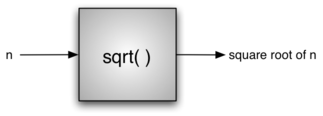
\includegraphics[width=3in]{images/blackbox.png}
\end{figure}

\section{什么是编程}

编程是将算法转换为编程语言的过程,以便被计算机执行。然而,编程语言有很多,计算的种类也不同,首先我们要有解决方案,没有算法就没有程序。


计算机科学不研究编程,但编程却是计算机科学家的重要能力。编程通常是表达解决方案的方式。因此,这种语言表现形式和创造它的过程成为该学科的基本部分。


算法描述了依据问题实例数据所产生的解决方案和产生预期结果所需的一套步骤。编程语言必须提供一种表示方法来表示过程和数据。为此,它提供了控制结构和数据类型。


控制结构允许以方便而明确的方式表示算法步骤。至少,算法需要执行顺序处理、决策选择和重复控制迭代。只要语言提供这些基本语句,它就可以表达算法。


计算机中的所有数据项都由一串一串的二进制数表示。为了让这些二进制串有意义,就需要有数据类型。数据类型为二进制数据提供解释,以便我们能够根据实际问题来思考数据。这些底层的内置数据类型(有时称为原始数据类型)为算法开发提供了基础。


例如,大多数编程语言为整数提供数据类型。内存中的二进制数据可以解释为整数,并且能给予一个我们通常与整数(例如 23,654 和 -19)相关联的含义。此外,数据类型还提供数据项参与的操作的描述。对于整数,诸如加法、减法和乘法的操作是常见的。我们期望数值类型的数据可以参与这些算术运算。


通常我们遇到的困难是问题及其解决方案非常复杂。由语言提供的简单的结构和数据类型,虽然可以表示复杂的解决方案,但在实际中却不好用。我们需要一些方法控制这种复杂性,以助于形成更好的解决方案。
\section{Python 数据结构的性能}

\begin{frame}\ft{\secname}
  你已经对大 O 记号和不同函数之间的差异有了了解。本节的目标是告诉你 Python 列表和字典操作的 大O 性能。


  给出一些基于时间的实验来说明每种数据结构的时间复杂度和使用这些数据结构的好处。

  重要的是了解这些数据结构的效率,因为它们是本课程实现其他数据结构所用到的基础模块。


  %本节中,我们将不会说明为什么是这个性能。在后面的章节中,你将看到列表和字典一些可能的实现,以及性能是如何取决于实现的。
\end{frame}



\subsection{列表}
\begin{frame}\ft{\subsecname}
  Python 的设计者在实现列表时有很多选择,每一种选择都可能影响列表操作的性能。

  对于常见的操作,对其实现进行了优化,以保证它们的处理非常快速。

  当然,他们还试图使较不常见的操作快速,当需要做出折衷时,较不常见的操作的性能通常牺牲以支持更常见的操作。
\end{frame}

\begin{frame}\ft{\subsecname}
  两个常见的操作是索引和分配到索引位置。无论列表有多大,这两个操作都需要相同的时间。当这样的操作和列表的大小无关时,它们是 $O(1)$。

\end{frame}

\begin{frame}\ft{\subsecname}
  
  另一种常见的操作是扩展列表,有两种方法可以创建更长的列表:
  \begin{itemize}
  \item append方法:时间复杂度为$O(1)$
  \item 拼接运算符:时间复杂度为$O(k)$,其中$k$ 是要拼接的列表的大小。
  \end{itemize}
  这对你来说很重要,因为它可以帮助你通过选择合适的工具来提高程序的效率。
\end{frame}

\begin{frame}\ft{\subsecname}

  观察四种不同的方式,以生成一个$0\~n$的列表。


  %1. 首先,我们将尝试一个 for 循环并通过创建列表,然后我们将使用 append 而不是拼接。接下来,我们使用列表生成器创建列表,最后,也是最明显的方式,通过调用列表构造函数包装 range 函数。 

  \lstinputlisting{code/list_compare.py}
\end{frame}

\begin{frame}[fragile]\ft{\subsecname}


为获取每个函数的执行时间,使用 Python 的 timeit 模块。
该模块允许 Python 开发人员在一致的环境中运行函数,并使用尽可能相似的操作系统的时序机制来进行跨平台时序测量。  

\end{frame}

\begin{frame}[fragile]\ft{\subsecname}
要使用 timeit,你需要创建一个 Timer 对象,其参数是两条 Python 语句:
\begin{enumerate}
\item 第一个参数是一个你想要执行时间的 Python 语句; 
\item 第二个参数是一个将运行一次以设置测试的语句。
\end{enumerate}
然后 timeit 模块将计算执行语句所需的时间。默认情况下,timeit 将尝试运行语句一百万次。 当它完成时,它返回时间作为表示总秒数的浮点值。


由于它执行语句一百万次,可以读取结果作为执行测试一次的微秒数。你还可以传递 timeit 一个参数名字为 number,允许你指定执行测试语句的次数。以下显示了运行我们的每个测试功能 1000 次需要多长时间。
\end{frame}

\begin{frame}[fragile]\ft{\subsecname}


\begin{lstlisting}
t1 = Timer("test1()", "from __main__ import test1")
print("concat ",t1.timeit(number=1000), "milliseconds")
t2 = Timer("test2()", "from __main__ import test2")
print("append ",t2.timeit(number=1000), "milliseconds")
t3 = Timer("test3()", "from __main__ import test3")
print("comprehension ",t3.timeit(number=1000), "milliseconds")
t4 = Timer("test4()", "from __main__ import test4")
print("list range ",t4.timeit(number=1000), "milliseconds")
\end{lstlisting}
\end{frame}

\begin{frame}[fragile]\ft{\subsecname}

\begin{lstlisting}[frame=no]
concat  6.54352807999 milliseconds
append  0.306292057037 milliseconds
comprehension  0.147661924362 milliseconds
list range  0.0655000209808 milliseconds
\end{lstlisting}

\end{frame}

\begin{frame}[fragile]\ft{\subsecname}

在上面的例子中,我们对 \lstinline|test1(), test2()| 等的函数调用计时,setup 语句可能看起来很奇怪,所以我们详细说明下。你可能非常熟悉 from ,import 语句,但这通常用在 python 程序文件的开头。在这种情况下,\lstinline|from __main__ import test1| 从 \lstinline|__main__| 命名空间导入到 timeit 设置的命名空间中。timeit 这么做是因为它想在一个干净的环境中做测试,而不会因为可能有你创建的任何杂变量,以一种不可预见的方式干扰你函数的性能。

\end{frame}

\begin{frame}[fragile]\ft{\subsecname}

从上面的试验清楚的看出,
\begin{enumerate}
	\item append 操作比拼接快得多;
	\item 列表生成器的速度是 append 的两倍;
	\item list函数是列表生成器的两倍。
\end{enumerate}
\end{frame}

%\begin{frame}[fragile]\ft{\subsecname}
%最后一点,你上面看到的时间都是包括实际调用函数的一些开销,但我们可以假设函数调用开销在四种情况下是相同的,所以我们仍然得到的是有意义的比较。因此,拼接字符串操作需要 6.54 毫秒并不准确,而是拼接字符串这个函数需要 6.54 毫秒。你可以测试调用空函数所需要的时间,并从上面的数字中减去它。
%现在我们已经看到了如何具体测试性能,见 Table2, 你可能想知道 pop 两个不同的时间。当列表末尾调用 pop 时,它需要 O(1), 但是当在列表中第一个元素或者中间任何地方调用 pop, 它是 O(n)。原因在于 Python 实现列表的方式,当一个项从列表前面取出,列表中的其他元素靠近起始位置移动一个位置。你会看到索引操作为 O(1)。python的实现者会权衡选择一个好的方案。
%\end{frame}

\begin{frame}[fragile]\ft{\subsecname}

\begin{table}[htbp]
\centering
\begin{tabular}{ll} \hline
操作&大 O 效率 \\\hline
\lstinline|index[]|         & $O(1)$ \\
\lstinline|index assignment|& $O(1)$ \\
\lstinline|append|          & $O(1)$ \\
\lstinline|pop()|           & $O(1)$ \\
\lstinline|pop(i)|          & $O(n)$ \\
\lstinline|insert(i,item)|  & $O(n)$ \\
\lstinline|del|             & $O(n)$ \\
\lstinline|iteration|       & $O(n)$ \\
\lstinline|contains(in)|    & $O(n)$ \\
\lstinline|get slice [x:y]| & $O(k)$ \\
\lstinline|del slice|       & $O(n)$ \\
\lstinline|set slice|       & $O(n+k)$ \\
\lstinline|reverse|         & $O(n)$ \\
\lstinline|concatenate|     & $O(k)$ \\
\lstinline|sort|            & $O(n\log n)$ \\
\lstinline|multiply|        & $O(nk)$ \\\hline 
\end{tabular}
\end{table}

\end{frame}

\begin{frame}[fragile]\ft{\subsecname}

作为一种演示性能差异的方法,我们用 \lstinline|timeit| 来做一个实验。我们的目标是验证从列表从末尾 pop 元素和从开始 pop 元素的性能。同样,我们也想测量不同列表大小对这个时间的影响。我们期望看到的是,从列表末尾处弹出所需时间将保持不变,即使列表不断增长。而从列表开始处弹出元素时间将随列表增长而增加。

\begin{lstlisting}
popzero = timeit.Timer("x.pop(0)", "from __main__ import x")
popend = timeit.Timer("x.pop()", "from __main__ import x")

x = list(range(2000000))
popzero.timeit(number=1000)
4.8213560581207275

x = list(range(2000000))
popend.timeit(number=1000)
0.0003161430358886719
\end{lstlisting}

这段代码展示了两种 pop 方式的比较。从第一个示例看出,从末尾弹出需要 0.0003 毫秒。从开始弹出要花费 4.82 毫秒。对于一个 200 万的元素列表,相差 16000 倍。
\end{frame}

%\begin{frame}[fragile]\ft{\subsecname}
%
%需要注意的几点,第一, \lstinline|from __main__ import x| , 虽然我们没有定义一个函数,我们确实希望能够在我们的测试中使用列表对象 x, 这种方法允许我们只计算单个弹出语句,获得该操作最精确的测量时间。因为 timer 重复了 1000 次,该列表每次循环大小都减 1。但是由于初始列表大小为 200万,我们只减少总体大小的 0.05\%。
%% Listing 4
%
%\end{frame}

\begin{frame}[fragile]\ft{\subsecname}

虽然我们第一个测试显示 \lstinline|pop(0)| 比 \lstinline|pop()| 慢, 但它没有证明 \lstinline|pop(0)| 是 $O(n)$, \lstinline|pop()|是 $O(1)$。要验证它,我们需要看下一系列列表大小的调用效果。
\begin{lstlisting}
popzero = Timer("x.pop(0)", "from __main__ import x") 
popend = Timer("x.pop()", "from __main__ import x")
print("pop(0)   pop()")
for i in range(1000000,100000001,1000000):
    x = list(range(i))
    pt = popend.timeit(number=1000)
    x = list(range(i))
    pz = popzero.timeit(number=1000)
    print("%15.5f, %15.5f" %(pz,pt))
\end{lstlisting}
\end{frame}

\begin{frame}[fragile]\ft{\subsecname}

下图展示了我们实验的结果,你可以看到,随着列表变长,pop(0) 时间也增加,而 pop() 时间保持非常平坦。这正是我们期望看到的 O(n)和 O(1)

\begin{figure}
\centering
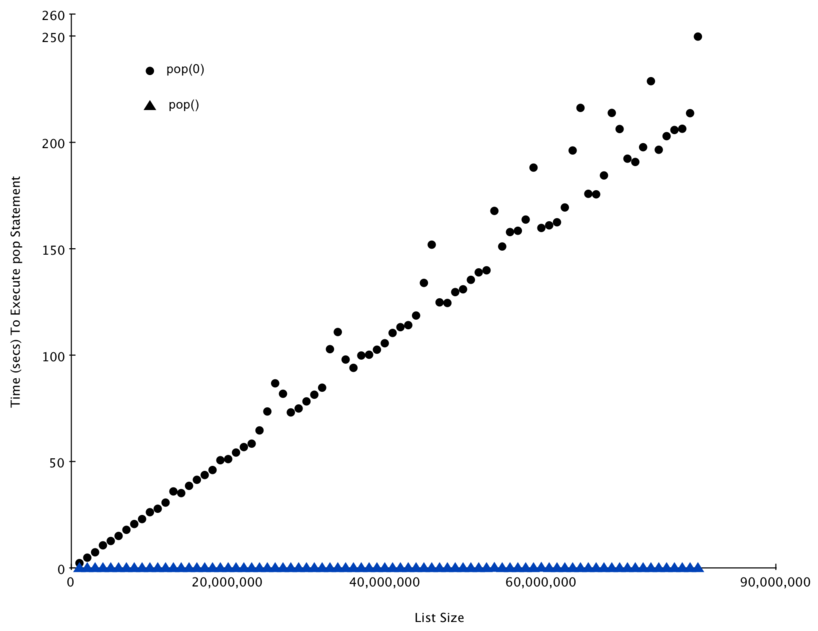
\includegraphics[width=4in]{images/poptime.png}
\end{figure}
\end{frame}

\subsection{字典}

\begin{frame}\ft{\subsecname}
  python 中第二个主要的数据结构是字典。
  
  
  与和列表不同,你可以通过键而不是位置来访问字典中的项目。在本书的后面,你会看到有很多方法来实现字典。
  
  字典的 get 和 set 操作都是 O(1)。
  
  另一个重要的操作是 contains,检查一个键是否在字典中也是 O(1)。
  
%  所有字典操作的效率总结在 Table3 中。关于字典性能的一个重要方面是,我们在表中提供的效率是针对平均性能。 在一些罕见的情况下,contains,get item 和 set item 操作可以退化为 O(n)。我们将在后面的章节介绍。
  \end{frame}

\begin{frame}[fragile]\ft{\subsecname}


\begin{table}[htbp]
  \centering
  \begin{tabular}{ll} \hline
    操作&大 O 效率 \\\hline
    \lstinline|copy|         & $O(n)$ \\
    \lstinline|get item     |& $O(1)$ \\
    \lstinline|set item|     & $O(1)$ \\
    \lstinline|delete item|  & $O(1)$ \\
    \lstinline|contains(in)| & $O(1)$ \\
    \lstinline|iteration|    & $O(n)$  \\\hline 
  \end{tabular}
\end{table}
\end{frame}

\begin{frame}[fragile]\ft{\subsecname}


我们现在来比较列表和字典之间的 contains 操作的性能。

在此过程中,我们将确认列表的 contains 操作符是 O(n),字典的 contains 操作符是 O(1)。

我们将在实验中列出一系列数字。然后随机选择数字,并检查数字是否在列表中。

如果我们的性能表是正确的,列表越大,确定列表中是否包含任意一个数字应该花费的时间越长。

%Listing 6 实现了这个比较。注意,我们对容器中的数字执行完全相同的操作。区别在于在第 7 行上 x 是一个列表,第9行上的 x 是一个字典。

\lstinputlisting{code/dict_time.py}
\end{frame}



\begin{frame}[fragile]\ft{\subsecname}

 

  \begin{figure}
    \centering
    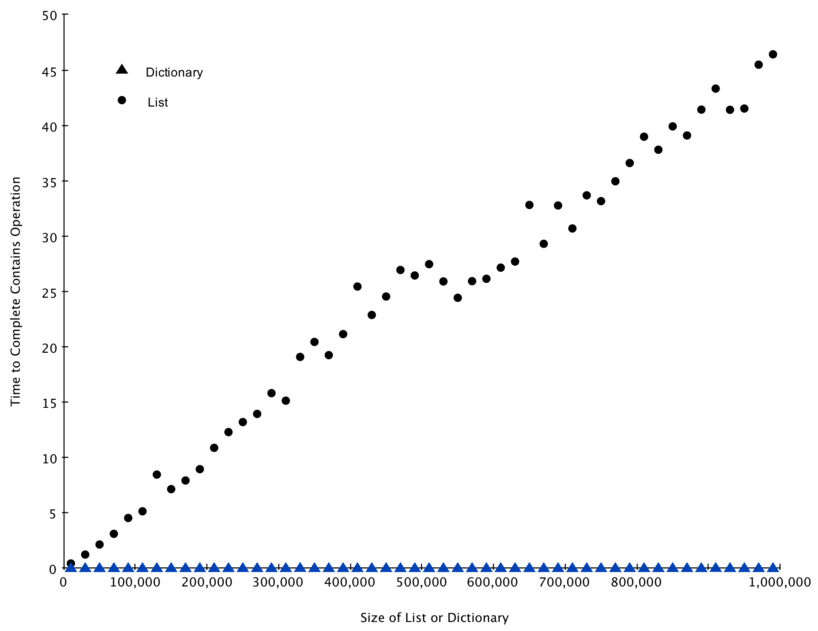
\includegraphics[width=4in]{images/dict_figure.png}
  \end{figure}
%由于 Python 是一种不断发展的语言,底层总是有变化的。 有关 Python 数据结构性能的最新信息可以在 Python 网站上找到。  

\end{frame}        


\begin{frame}[fragile]\ft{\subsecname}


上图展示了前一段的结果。你可以看到字典一直更快。 对于最小的列表大小为10 000个元素,字典是列表的89.4倍。

对于最大的列表大小为990 000 个元素。字典是列表的11,603倍!

你还可以看到列表上的contains运算符所花费的时间与列表的大小成线性增长。

这验证了列表上的contains运算符是 O(n) 的断言。

还可以看出,字典中的 contains 运算符的时间是恒定的,即使字典大小不断增长。


事实上,对于字典大小为10 000个元素,contains操作占用0.004毫秒,对于字典大小为990 000个元素,它也占用0.004毫秒。
\end{frame}
\end{document}
